% !TEX root = ../TechProject.tex

\graphicspath{{Chapter5/}}


\chapter{Experiment}


As explained in the hypothesis. a music recommendation system that uses MixesDB as a dataset was made. An experiment was ran to see if it garners appropriate results, and will help answer the following question:
\\
\\
\textit{Is the proposed method a suitable solution to automate recommendations of songs suitable for adding to a given DJ set?}.
\\

To evaluate the quality of a recommendation system, R-Precision is often used as a performance metric. 
\\

\section{R-Precision}

\begin{equation}
	R-Precision = \frac{|G\cap R_{1:|G|}|}{|G|}
\end{equation}
\\\\
The R-precision is the amount of found tracks that were originally in the mix divided by the number of known missing tracks.

The idea for the testing came from the million playlist dataset from Spotify  that was used for the 2018 Recsys Convention\citep{aicrowd_aicrowd_2023}. At this convention, competing teams would make a recommendation system out of the dataset. To tests its quality, a challenge dataset, which contained many modified playlists, was used to test the models.

It is important to note that there is a considerable difference in the number of DJ sets/playlists between the MixesDB dataset and the Spotify one. The MixesDB dataset contains over 9800 DJ sets, while the Spotify dataset contains 1,000,000 playlists. It is also essential to discuss the differences in definition of a playlist and a DJ set. A playlist being a collection of songs, regardless of cohesion or song count, while a DJ set is typically a seamless mix of songs that can vary in length from 8 hours to no less than 20 minutes.

The top 10 scoring models from the convention have R-Precision values ranging from 0.21 to 0.22. Given the differences in dataset size and task, aiming for an average R-Precision value of 0.171, slightly lower than the top-performing models, would be appropriate. Achieving this value would rank the model within the top 30 models trained by members of the public on the given spotify dataset \citep{aicrowd_aicrowd_2023}. This approach allows for a fair comparison between the different systems and considers the unique characteristics of the dataset and task at hand. 

As the dataset utilized with the proposed model was obtained from MixesDB, it was necessary to devise a customized approach for the preparation of the evaluation set.

\section{Preparing Evaluation Set}
During the evaluation phase of the million playlist challenge, the quality of a given applications trained on this dataset was assessed through a range of methods that involved analysing both missing and recommended songs. In order to effectively compare different applications, it was essential to create a standardised evaluation set that incorporated aspects of the Spotify data set, which could show the applications that can recommend songs that were featured in the playlists originally.

\begin{figure}[H]
	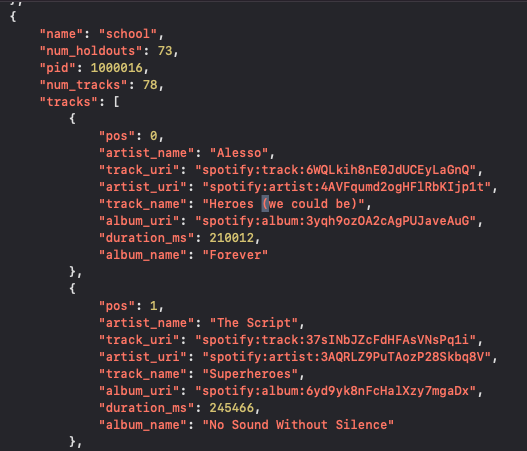
\includegraphics[scale=0.5]{images/spotify_challenge_set}
	\centering
	\caption{Screenshot of spotify challenge set. \citep{aicrowd_aicrowd_2023}} 
\end{figure}

The Spotify challenge set consisted of 10,000 playlists with varying numbers of input songs, ranging from 0 to 100 tracks. For each of these playlists, Spotify requested 500 track recommendations from the participating teams \citep{aicrowd_aicrowd_2023}. However, due to the relatively smaller scale of the dataset and difference between playlists and DJ sets under consideration, various aspects of this challenge set had to be downscaled to maintain the academic rigour of the study. For instance, the range of input songs was considerably narrower, as DJ sets typically have a minimum length of 10 tracks, compared to playlists that can have varying lengths.

To ensure the feasibility of finding all songs in the evaluation set, an additional criterion was applied, whereby each song had to have a total play count of at least 5. This value was chosen to ensure that each song in the set would likely be found in the training set. Furthermore, the input and missing songs were divided in a standardized manner, with 20\% of the songs allocated as missing songs, and the remaining 80\% as input songs. Overall, the creation of the evaluation set was a crucial aspect of the study, ensuring that the assessment of the applications was based on a consistent and standardized evaluation framework. The output value for the application was also changed to 100 work better with the smaller dataset.

The making of the evaluation set was coded in python using the pandas library, the code for this can be found on GitHub\footnote{\url{https://github.com/HarveyPrew/DJSetFiller/blob/main/src/DJSetFiller/prepare_evaluation_set.py}}.
\\
\begin{figure}[H]
	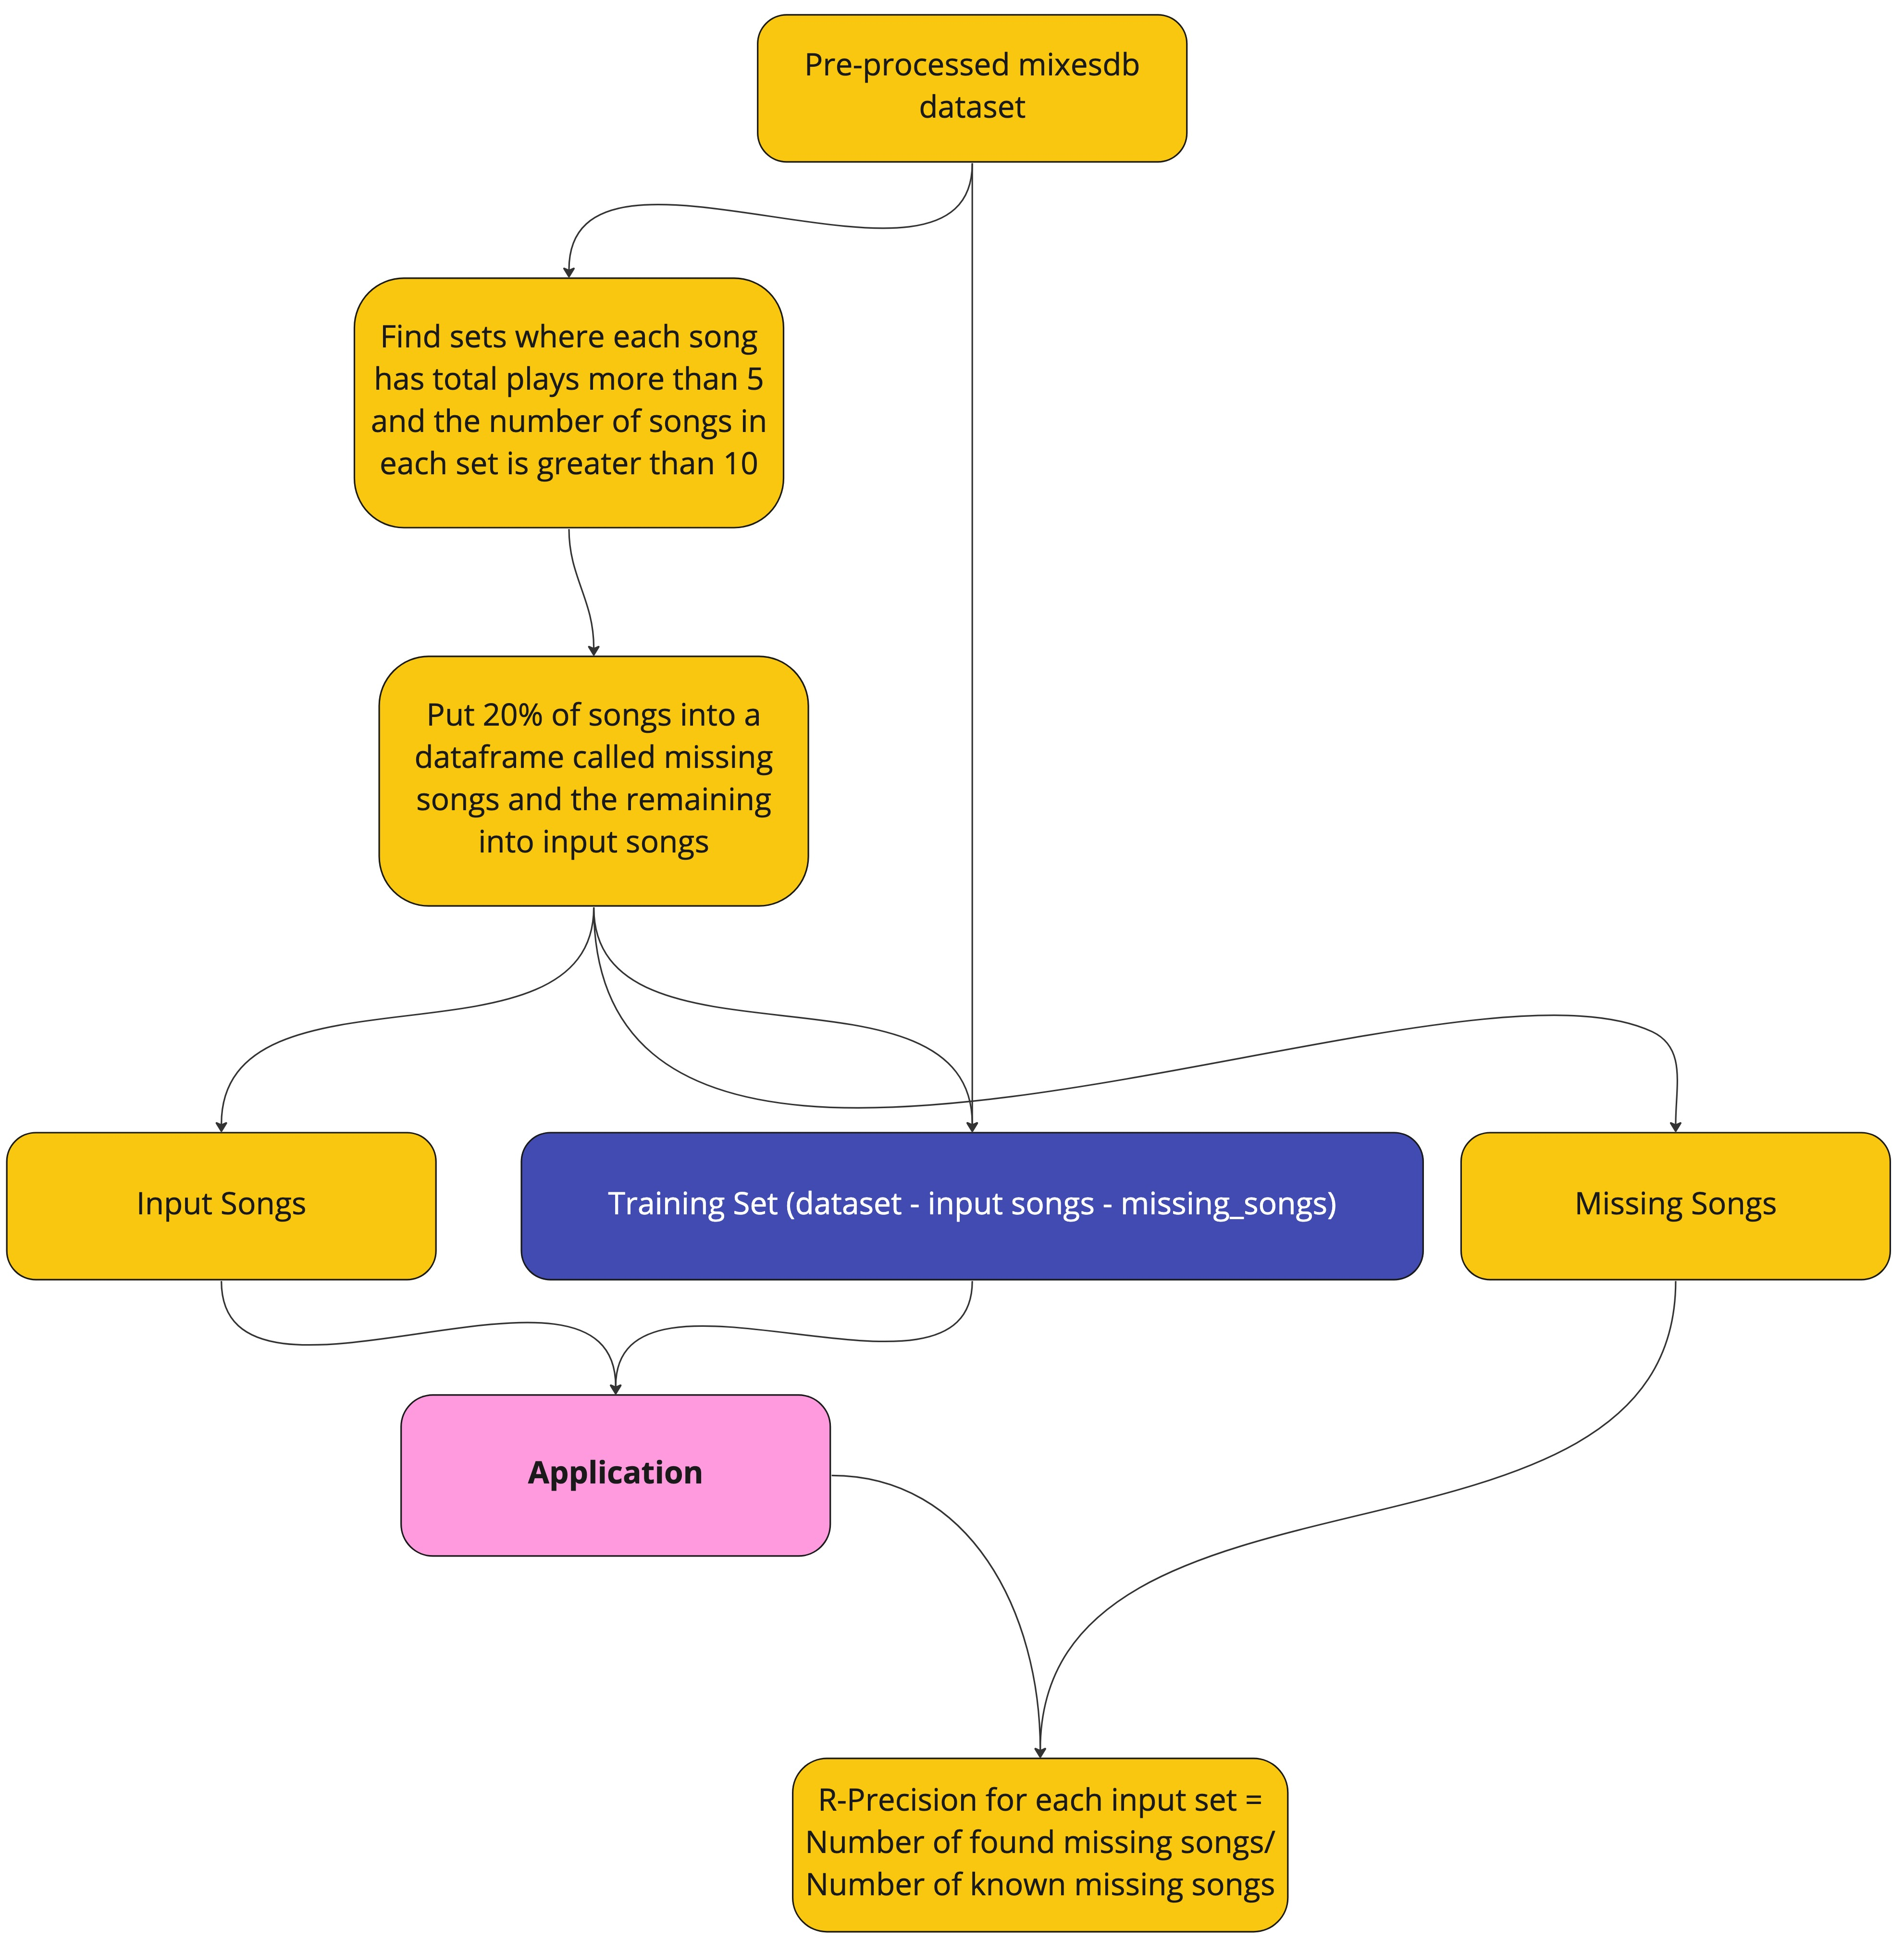
\includegraphics[scale=0.1]{images/evaluation_set_app_flow}
	\centering
	\caption{Application flow of the creation of the evaluation set} 
\end{figure}

\section{Experiment Variables}

As mentioned in chapter 5, the proposed application utilizes the ALS algorithm to generate a preliminary set of suggestions. This algorithm is based on matrix factorization, where the latent factors are derived from the training dataset to identify similar songs. The selection of an appropriate value for latent factors is crucial in ensuring the optimal performance of the algorithm. A value that is too low may yield results that are too random, while a value that is too high may lead to an excessive focus on specific items. To identify the ideal value for latent factors, it is necessary to conduct an  investigation where the latent factors will be the independent variable, and the average R-precision value will be the dependent variable. Furthermore, an examination on how changes to the parameters of the evaluation set, particularly larger DJ sets, impact the R-Precision value. From there, the R-precision value  is then compared to the highest performing recommendation systems that use the Spotify Dataset, to see if the DJ set focused recommender can compare to industry standard algorithms.

The average R-Precision got tested on varying latent factor values, and when the highest was found, the selection of input DJ sets was altered, choosing DJ sets with a higher amount of songs. This was done to further explore what size an input gets the best results. The experiment was ran on a 16GB 2020 MacBookPro.

